\chapter{The KZM across a first-order phase transition in a spin-1 BEC}


\section{Introduction}

\section{The Kibble-Zurek mechanism}\label{sec:the-KZM}
Consider a system that undergoes a spontaneous breaking of symmetry when a
control parameter, $\lambda$, is ramped across a phase transition that occurs
at the critical point, $\lambda_c$.
A continuous second-order phase transition can be characterized by a divergence
of the equilibrium correlation length
\begin{equation}
    \xi(\epsilon) = \frac{\xi_0}{|\epsilon|^z},
\end{equation}
and an equilibrium relaxation time
\begin{equation}
    \tau(\epsilon) = \frac{\tau_0}{|\epsilon|^{z\nu}},
    \label{eq: equil-relax-time}
\end{equation}
where
\begin{equation}
    \epsilon - \frac{\lambda_c - \lambda}{\lambda_c}
\end{equation}
is a reduced distance parameter.
The system is initially prepared in a high-symmetry phase $(\epsilon < 0)$ but 
breaks that symmetry as the critical point is crossed $(\epsilon > 0)$.
In the above equations, the exponents $z$ and $\nu$ are the dynamical and
correlation length critical exponents, respectively.
These exponents are determined by the universality class of the phase
transition, and different systems belonging to the same universality class share
the same critical exponents.
\textcolor{red}{Examples of different exponents for different classes? Links
to refs that calculate values?}
In contrast, the constants $\xi_0$ and $\tau_0$ are determined by the
microscopic details of the system. \par
The KZM describes the dynamics of crossing the critical point when $\lambda$ 
is continually varied.
We assume the form of a linear quench, such that the control parameter can be
written as
\begin{equation}
    \lambda(t) = \lambda_c - \epsilon(t),
\end{equation}
which is symmetric about the critical point so that the reduced distance
parameter is defined as
\begin{equation}
    \epsilon(t) = \frac{t}{\tau_Q}
    \label{eq: time-dependent-epsilon}
\end{equation}
for a quench time $\tau_Q$.
Here, $t \in [-\tau_Q, \tau_Q]$, where the critical point is reached at $t=0$.
From Eq.~\eqref{eq: equil-relax-time}, we see that far from the critical point
($|\lambda| \gg \lambda_c \implies |\epsilon| \gg 1$ ) the equilibrium
relaxation time is small compared to the time taken to reach the critical point
[Eq.~\eqref{eq: time-dependent-epsilon}]; which implies the dynamics is
adiabatic.
Conversely, as we approach the critical point ($\epsilon \rightarrow 0$), the
equilibrium relaxation time diverges and the dynamics of the system freeze,
known as critical slowing down.
As the critical point is passed, the system can once again resume the adiabatic
dynamics as the equilibrium relaxation time no longer diverges.
This then splits the dynamics into three parts as $\epsilon(t)$ is ramped from
$\epsilon(t) < 0 $ to $\epsilon(t) > 0$: adiabatic, frozen, and adiabatic again
(see Fig.~\ref{fig: adiabatic-impulse} for a schematic representation).
\begin{figure}
    \centering
    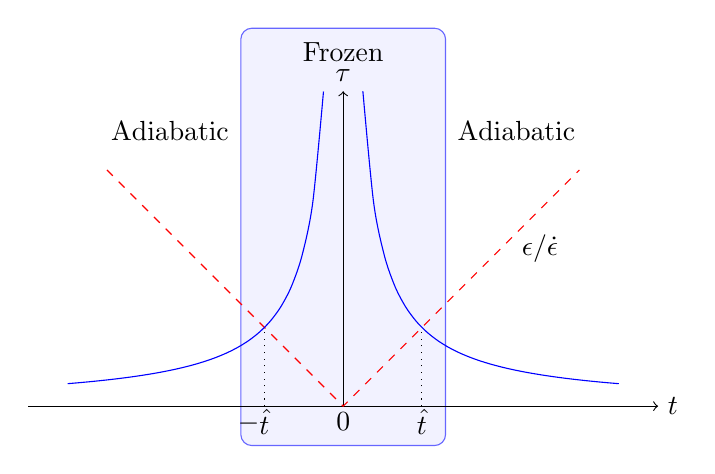
\begin{tikzpicture}
        \filldraw[color=blue!60, fill=blue!5, rounded corners] (-1.3, -0.5) 
        rectangle (1.3, 4.8);
        \draw[->] (-4, 0) -- (4, 0) node[right] {$t$};
        \draw[->] (0, 0) -- (0, 4) node[above] {$\tau$};
        \draw[scale=1, domain=-3:3, dashed, variable=\x, red] plot 
        ({\x}, {abs(\x)});
        \draw[scale=1, domain=0.25:3.5, smooth, variable=\x, blue] plot 
        ({\x}, {\x^(-1)});
        \draw[scale=1, domain=-3.5:-0.25, smooth, variable=\x, blue] plot 
        ({\x}, {abs(\x^(-1))});
        \node at (1, -0.2) {$\hat{t}$};
        \node at (-1, -0.2) {$\hat{t}$};
        \node at (-1.2, -0.22) {$-$};
        \draw[dotted] (1, 0) -- (1, 1);
        \draw[dotted] (-1, 0) -- (-1, 1);
        \node at (0, 4.5) {Frozen};
        \node at (2.5, 2) {$\epsilon/\dot{\epsilon}$};
        \node at (2.2, 3.5) {Adiabatic};
        \node at (-2.2, 3.5) {Adiabatic};
        \node at (0, -0.2) {$0$};
    \end{tikzpicture}
    \caption{A schematic representation of the dynamics of a system during a
    linear quench. The system starts in a high-symmetry phase ($t>0$) and is
    quenched across a critical point to a low symmetry phase ($t < 0$) by the
    reduced control parameter (red dashed line) $\epsilon(t)=t/\tau_q$. As
    the critical point is approached, the equilibrium relaxation time
    (blue line) diverges, and the order parameter can no longer follow the 
    ground state, leading to frozen dynamics in the interval
    $t \in [-\hat{t}, \hat{t}]$}. Figure reproduced from~\cite{delCampo2013}.
    \label{fig: adiabatic-impulse}
\end{figure}

The extent of the frozen region can be estimated by comparing the equilibrium
relaxation time with the time elapsed after the critical point
\begin{equation}
    \tau(t) \approx \left|\frac{\epsilon}{\dot{\epsilon}}\right|=t.
\end{equation}
Solving the above equation yields the freeze-out time $\hat{t}$:
\begin{equation}
    \hat{t} \sim (\tau_0\tau_Q^{z\nu})^{\frac{1}{1+z\nu}}.
    \label{eq: freeze-out-time}
\end{equation}
In the time interval $t \in [-\hat{t}, \hat{t}]$, the order parameter cannot
keep up with the change of the control parameter and therefore lags
behind the equilibrium value, $\hat{\epsilon}$, defined as
\begin{equation}
    \hat{\epsilon} \equiv |\epsilon(\hat{t})| \sim 
    \left(\frac{\tau_0}{\tau_Q}\right)^\frac{1}{1+z\nu}.
\end{equation}

As the symmetry of the system is broken, disconnected regions form which
have a spontaneously chosen value of the order parameter.
The size of these domains is set by the value of the equilibrium correlation
length at $\hat{t}$:
\begin{equation}
    \hat{\xi} \equiv \xi(\hat{t}) 
    = \xi_0 \left(\frac{\tau_Q}{\tau_0}\right)^\frac{\nu}{1 + z\nu}.
    \label{eq: KZM-domain-size}
\end{equation}
Using this length scale, we can predict the density of defects, $n_d$, by
the ratio of the size of the defects $\hat{\xi}^d$ and the size of the domains
$\hat{\xi}^D$
\begin{equation}
    n_d \sim \frac{\hat{\xi}^d}{\hat{\xi}^D}=\frac{1}{\xi_0^{D-d}}
    \left(\frac{\tau_0}{\tau_Q}\right)^{(D-d)\frac{\nu}{1 + z\nu}},
\end{equation}
where $D$ and $d$ are the dimensions of space and the defects, respectively.
In a 3D superfluid containing quantum vortices, $D=3$ and $d=1$.
If we assume the mean-field predictions for the exponents
($z=2$, $\nu=\frac{1}{2}$), then the density of defects scales as
\begin{equation}
    n_d \propto \tau_Q^{-\frac{1}{2}}.
\end{equation}
\textcolor{red}{Experimentally there have been different observations giving
$n_d \propto \tau_Q^{-1/3}$. You can use `Model-F' exponents $\nu=3/2, z=3/2$
in the above equation to recover this result.}

\subsection{The generalized Kibble-Zurek mechanism}

\subsection{The Kibble-Zurek mechanism in spin-1 BECs}
As shown in \textcolor{red}{relevant section}, there are four ground states
phases of spin-1 Bose-Einstein condensates; namely, the ferromagnetic,
antiferromagnetic, polar, and broken-axisymmetry phases, where each ground
state phase has an associated symmetry.
The Kibble-Zurek mechanism can be studied in spin-1 BECs by considering how
the change of a control parameter causes the order parameter to change from 
one ground state to another.
As it does this, the symmetry of the system is spontaneously broken, and hence
the Kibble-Zurek theory can be applied.

Spin-1 BECs support numerous first- and second-order phase transitions
when the linear, $p$, or quadratic, $q$, Zeeman shifts are
ramped across a critical point~\cite{Kawaguchi2012}.
A second-order transition is characterised by the derivative of the energy with
respect to $p$ and $q$ change continuously across the transition.
For example, in a spin-1 BEC with polar interactions, the ground state is in
the antiferromagnetic state for $|p|/c_2n<1$ and $q/c_2n<0$ which has energy
$\epsilon = q - \frac{p^2}{2c_2n}-\frac{1}{2}c_0n$.
As $p$ is ramped across the critical point at $|p|/c_2n=1$, the ground state
becomes the ferromagnetic state with energy
$\epsilon = -p + q + \frac{1}{2}(c_0 - c_2)n$.
We see the derivatives of the two energies are continuous at the critical point,
and hence this is a second-order phase transition.

\section{Broken-axisymmetry to ferromagnetic quench}
The KZM typically concerns second-order phase transitions. However, recent
work has been conducted in condensed matter systems which investigate
the KZM across first-order transitions~\cite{Qiu2020}.
We aim to extend this research and present results for
the first-order transition between the broken-axisymmetry and
ferromagnetic phases.

We start from the broken-axisymmetry (BA) wavefunction with $p=0$
\begin{equation}
    \psi_{\pm 1} = \frac{\sqrt{2}}{4}\sqrt{2 - Q(t)}, \qquad
    \psi_0 = \frac{1}{2}\sqrt{2 + Q(t)},
    \label{eq: BA-initial-wavefunction}
\end{equation}
where $Q(t)=q(t)/|c_2|n$.
The BA wavefunction is the ground state for $c_2 < 0$ and $0 < Q < 2$.
There exists a critical point at $Q=0$ where the ground state changes from
the BA phase to the ferromagnetic phase.
We perform 1D simulations on a grid of $N_x = 16384$ grid points with a grid
spacing of $\Delta_x = 0.125$.
We perturb the initial BA state by adding small noise, $\delta_m$, to each
component where $|\delta_m| \ll 1$.
We generate the real and imaginary parts of $\delta_m$ for each grid point
using the probability distribution
$p(x) = e^{-x^2/2\sigma^2}(\sqrt{2\pi}\sigma)^{-1}$.
We choose $\sigma=10^{-4}$ so that we start close to the BA ground state.

\section{Phase boundaries in the ferromagnetic phase}
As the system is quenched across the critical point at $Q=0$, the ground state
changes to the ferromagnetic phase.
The order parameter for this phase takes the form $\zeta=(1,0,0)^T$ or 
$\zeta=(0,0,1)^T$ depending on the orientation of the spin.
From Eq.~\eqref{eq: BA-initial-wavefunction} we have
$\psi_{\pm 1} = \frac{1}{2}$ and $\psi_0 = \frac{\sqrt{2}}{2}$ at $Q=0$.
The question that remains is: Which state will the system choose after
the critical point is passed?

\begin{figure}[tb]
    \centering
    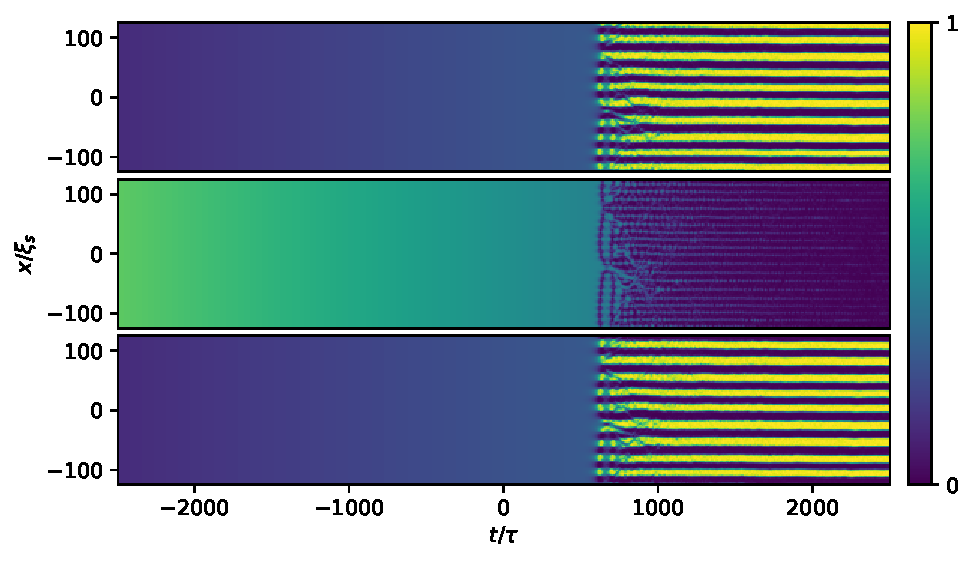
\includegraphics[width=\textwidth]{gfx/ch-spin1/BA-FM_all_densities.pdf}
    \caption{Plots of $|\psi_1|^2$ (top) $|\psi_0|^2$ (middle) and
    $|\psi_{-1}|^2$ (bottom) as a function of time for a $256\xi_s$
    spatial subregion of the condensate for $\tau_Q=2500\tau$.}
    \label{fig: BA-FM-densities}
\end{figure}
Fig.~\ref{fig: BA-FM-densities} shows the full evolution of the density of each
component for a quench time $\tau_Q=5000\tau$.
As the Zeeman shift is quenched, we see the density of the $\psi_0$ component
linearly decrease as the $\psi_{\pm 1}$ components increase.
After the critical point at $t/\tau=0$ is passed there is a freeze-out time
(see Sec.~\ref{sec:the-KZM}) before the system crosses into the ferromagnetic
phase.
During this new phase, we see the formation of ferromagnetic domain walls
(characterised by the bright density peaks) in the $\psi_{\pm 1}$ components as
the order parameter adjusts to the new ground state.
These domains are spatially separated and where there is zero density in one of
the components, there is maximal density in the other so that overall the total
density $n=\sum_m\psi_m^*\psi_m$ is uniform.

The KZM predicts in Eq.~\eqref{eq: KZM-domain-size} that the size of the domains
grow as the quench time increases.
\begin{figure}[tb]
    \centering
    \begin{subfigure}{0.45\textwidth}
        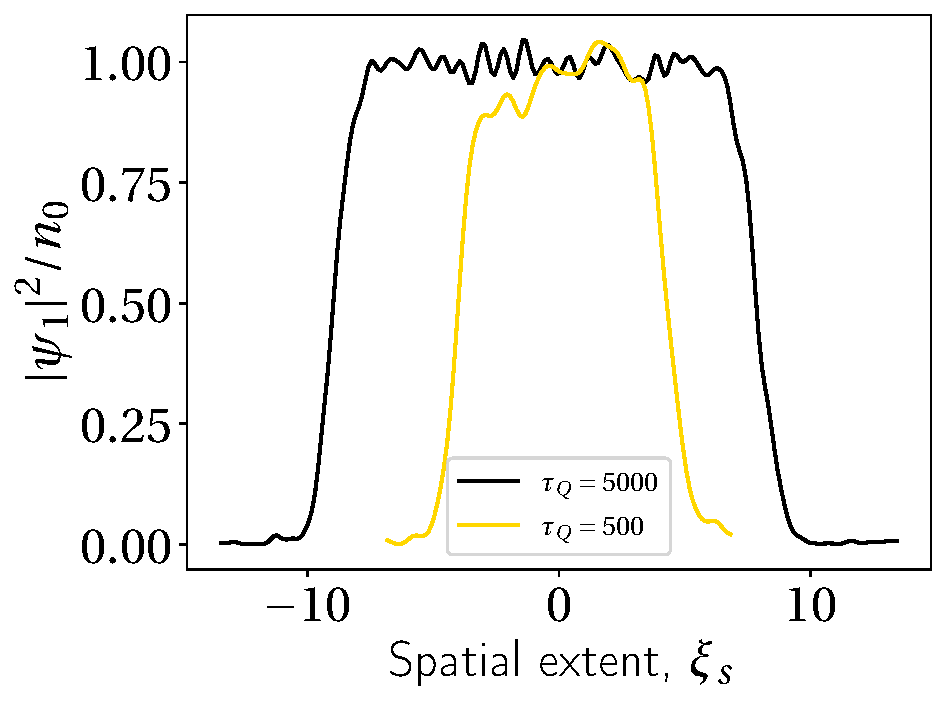
\includegraphics[width=\textwidth]{gfx/ch-spin1/BA-FM_domain_width.pdf}
        \caption{}
        \label{fig: BA-FM-domain-width-comparison}
    \end{subfigure}
    \begin{subfigure}{0.45\textwidth}
        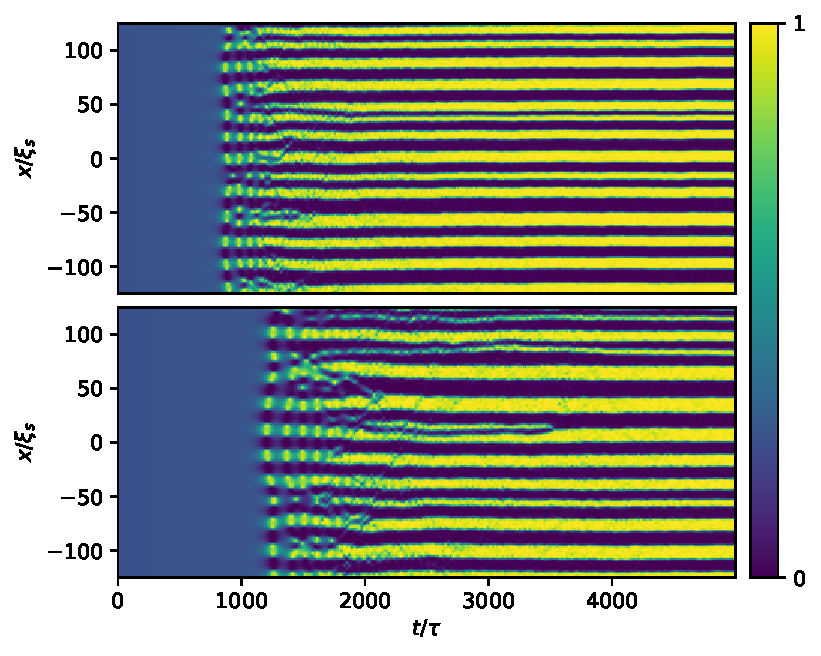
\includegraphics[width=\textwidth]{gfx/ch-spin1/BA-FM_domain_onset.pdf}
        \caption{}
        \label{fig: BA-FM-domain-onset}
    \end{subfigure}
    \caption{(a): Density profile of the $\psi_1$ component across an average
    domain in a simulation with $\tau_Q=2500\tau$ (black line) and
    $\tau_q=10000$ (red line).
    (b): Time evolution of $|\psi_1|^2$ for a $256\xi_s$ spatial subregion
    for $\tau_Q=5000\tau$ (top) and $\tau_Q=10000\tau$ (bottom).}
\end{figure}
Fig.~\ref{fig: BA-FM-domain-width-comparison} shows the average domain size
for two different simulations with $\tau_Q=2500$ and $\tau_Q=10000$.
We see that the longer quench time produces domains that have a
larger width than those of faster quenches, supporting the Kibble-Zurek theory.
In addition, we plot the time evolution of $|\psi_1|^2$ for $\tau_Q=5000$ and
$\tau_Q=10000$ in Fig.~\ref{fig: BA-FM-domain-onset}.
We see the ferromagnetic domain formation is delayed in the simulation
with a longer quench time, which supports the prediction in
Eq.~\eqref{eq: freeze-out-time}.

One can count the number of ferromagnetic domains in the system and see the
dependence on $\tau_Q$.
To do this, we developed a numerical algorithm that counts the number of
density peaks in each component and sums the result to give the total number of
domains, $N_d$.
We calculate this quantity at time $t/\tau=\tau_Q/2$ in each simulation, to
ensure that the domains are frozen and avoid the early-time coarsening
taking place which could affect the total number of domains present.
\begin{figure}
    \centering
    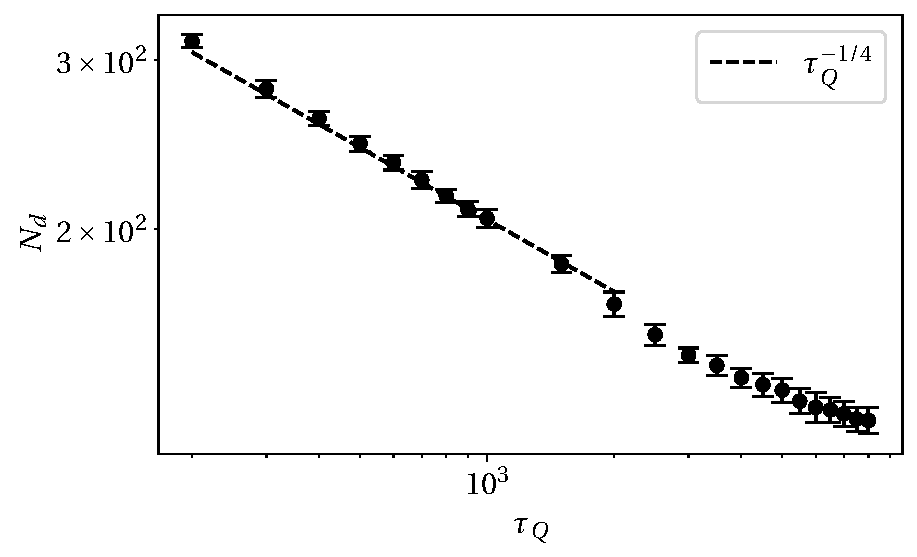
\includegraphics[width=0.65\textwidth]{gfx/ch-spin1/FM_domains_scaling.pdf}
    \caption{The number of ferromagnetic domains as a function of the
    quench time. Each point represents 50 simulations and the
    errorbar gives one standard deviation. Overlaid are the scaling lines
    $\tau_Q^{-1/3}$ (black dashed line) and $\tau_Q^{-1/5}$ (red dotted line).}
    \label{fig: FM-domains-scaling}
\end{figure}
In Fig.~\ref{fig: FM-domains-scaling} we plot the total number of domains
as a function of the quench time with 50 ensemble runs for each simulation.
We see that there is not a uniform scaling throughout all quench times tested.
Faster quenches indicate a steeper power-law scaling of the number of domains
that approaches $N_d\sim\tau_Q^{-1/3}$.
As the quench time slows, a deviation from this scaling takes place at
approximately $\tau_Q\approx 3\times10^3\tau$, where the scaling of the domains
approaches $N_d\sim\tau_Q^{-1/5}$.
\textcolor{red}{I guess the question now is: why is there a deviation?
Is the larger domain size (due to slower quench times) affecting the scaling?
Is it a consequence of the grid size? Can the $1/3$ scaling be linked to KZ
theory?}

\section{Power-law scaling near the critical point}

\subsection{Bogoliubov theory in spin-1 BECs}
Bogoliubov analysis is an indispensable tool for determining the stability of
states within BEC systems [REFS to Bogoliubov papers?].
\textcolor{red}{I plan to have details regarding the derivation of the
Bogoliubov energies etc. but for now I will just list them for the BA phase.}

The Bogoliubov energies for mode $\vb{k}$ and component $m$ for the
broken-axisymmetry phase are:
\begin{equation}
    E_{\vb{k}, {f_z}} = \sqrt{\epsilon_{\vb{k}}(\epsilon_{\vb{k}} + q)},
    \label{eq: zero-mode-energy}
\end{equation}
\begin{equation}
    E_{\vb{k}, \pm} = \sqrt{\epsilon_{\vb{k}} + n(c_0 + c_2)\epsilon_{\vb{k}} 
    + 2(c_2n)^2(1 - \tilde{q}^2) \pm \Lambda_{\vb{k}}},
    \label{eq: pmone-mode-energy}
\end{equation}
where $\epsilon_{\vb{k}} = \hbar^2\vb{k}^2 / 2M$, $\tilde{q} = -q/(2c_2n)$ and
\begin{equation}
    \Lambda_{\vb{k}} = \sqrt{[(c_0+3c_2)n\epsilon_{\vb{k}} 
    + 2(c_2n)^2(1-\tilde{q}^2)] 
    - 4c_2(c_0+2c_2)n^2\tilde{q}^2\epsilon_{\vb{k}}^2}.
\end{equation}
The imaginary part of the above energies becoming non-zero signals an
instability present in that respective mode.
\begin{figure}[tb]
    \centering
    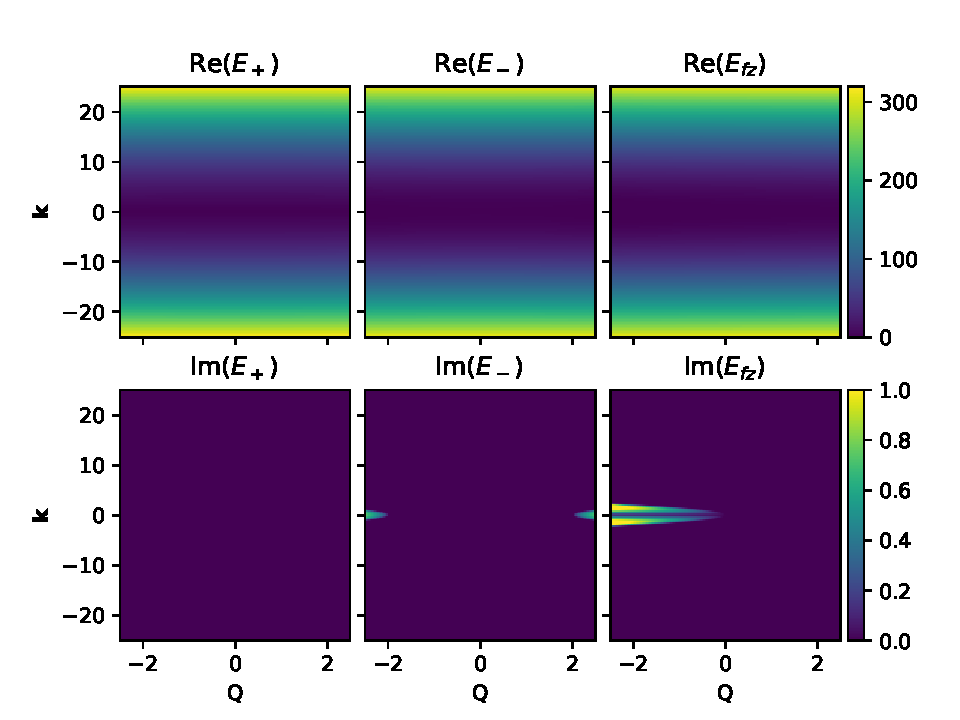
\includegraphics[width=\textwidth]{gfx/ch-spin1/dens_spin_energies.pdf}
    \caption{Real and imaginary parts of the energies in
    Eqs.~\eqref{eq: zero-mode-energy}-\eqref{eq: pmone-mode-energy} in a
    parameter space of mode $\vb{k}$ and $Q=q/|c_2|n$.}
    \label{fig: dens-spin-energies}
\end{figure}
Fig.~\ref{fig: dens-spin-energies} shows the real and imaginary parts of the
above energies in a parameter space of $(\vb{k}, Q)$.
Firstly, one sees the growth of the $\mathrm{Im}(E_{\vb{k}, -})$ energy
when $|Q| > 2$.
When $Q>2$, the lowest energy of the system is achieved by having the condensate
become polar ($\zeta^P=(0,1,0)^T$).
\textcolor{red}{Why is there an instability for $Q<-2$? Did we ever put our
finger on this? Mirkhalaf~\cite{Mirkhalaf2021} has a plot that shows the
critical point between the BA to FM phase is at $Q = -2$. We're 
seeing the transition at $Q=0$ however. In our simulations we only quench
from Q=1 to Q=-1, should we just include that range instead?}
Secondly, we see the growth of the $\mathrm{Im}(E_{\vb{k}, {f_z}})$ mode when
$Q<0$.
This signals the change from the broken-axisymmetry phase to the ferromagnetic
phase and hence is the relevant mode in our system.

\subsection{Observation of power-law scaling}
Since we know the relevant unstable mode within our system, we can investigate
power-law scaling near the critical point.
To begin, we start with the fluctuation operator associated with the
Bogoliubov spectrum $E_{\vb{k}, fz}$
\begin{equation}
    \hat{a}_{\vb{k}, {f_z}} = \frac{1}{\sqrt{2}}(\hat{a}_{\vb{k}, 1} 
    - \hat{a}_{\vb{k}, -1}),
    \label{eq: fz-fluctuation-operator}
\end{equation}
where $\hat{a}_{\vb{k}, \pm1}$ is the annihilation operator for a spin-1 boson
with wave number $\vb{k}$ in component $m=\pm1$.
\begin{figure}[tb]
    \centering
    \begin{subfigure}{0.45\textwidth}
        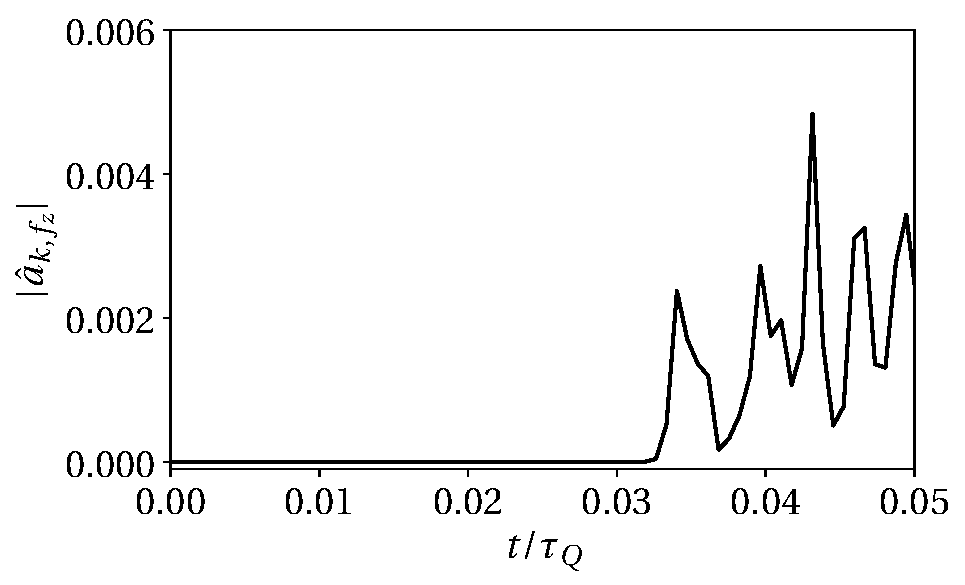
\includegraphics[width=\textwidth]
        {gfx/ch-spin1/1d_BA-FM_5000_fluctuation_diff.pdf}
        \caption{}
        \label{fig: fluctuation-diff}
    \end{subfigure}
    \begin{subfigure}{0.45\textwidth}
        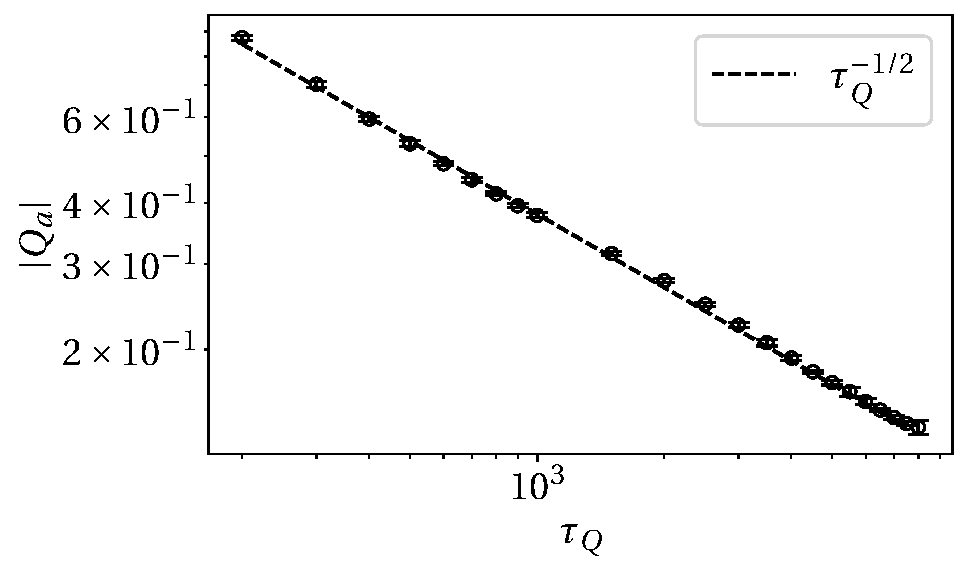
\includegraphics[width=\textwidth]{gfx/ch-spin1/BA-FM_Qa_scaling.pdf}
        \caption{}
        \label{fig: Q_a-scaling}
    \end{subfigure}
    \caption{(a): The modulus of the fluctuation operator in
    Eq.~\eqref{eq: fz-fluctuation-operator} for $\vb{k}=1$ and $\tau_Q=5000$.
    The plot shown is obtained by averaging over all runs in the ensemble.
    (b): The critical value $Q_a$ as a function of the quench time.
    }
\end{figure}
Fig.~\ref{fig: fluctuation-diff} shows the above quantity for a quench time
of $\tau_Q=5000$ with $\vb{k}=1$.
The quantity remains zero until after the critical point is passed, where
a rapid period of growth occurs.
This onset of this growth corresponds to the ferromagnetic domains forming
within the system (see Fig.~\ref{fig: BA-FM-densities}).
Motivated by previous work~\cite{Damski2007, Qiu2020}, we define a time,
$\hat{t}$, which is the time when $|\hat{a}_{\vb{k}, {f_z}}|$ first exceeds
1\% of its maximum value: $|\hat{a}_{\vb{k}, {f_z}}(\hat{t})| =
0.01\times \mathrm{max}|\hat{a}_{\vb{k}, {f_z}}(t)|$.
For the system in Fig.~\ref{fig: fluctuation-diff}, we obtain $\hat{t}=598\tau$.
Using this time, we can extract the critical value of $Q$ that this growth
occurs at, $Q(\hat{t}) = Q_a$.
Fig.~\ref{fig: Q_a-scaling} shows $Q_a$ as a function of the quench time.
We see a clear power-law scaling of $Q_a \propto \tau_Q^{-\frac{1}{2}}$ for
all values of $\tau_Q$ tested.
This exponent differs from observed results in previous works investigating
second-order phase transitions~\cite{Damski2007, Anquez2016, Swislocki2013}
where an exponent of $-1/3$ is observed.
Our observation of a $-1/2$ exponent signifies a deviation from
the Kibble-Zurek theory which appears to be a consequence of our transition
being first-order.

\subsection{Deriving the observed power-law scaling}
We wish to rigorously derive the scaling obtained in
Fig.~\ref{fig: Q_a-scaling}.
We follow a process similar
\section{Other quench results? 2D?}
